% Schematicky podle P4, PDF s. 40–41; hodnoty a názvy podle tabulky na s. 40.
% Osa teploty není číselně kalibrována: teploty závisí na složení skla.
\documentclass[border=3mm]{standalone}
\usepackage{fontspec,amsmath,tikz}
\setsansfont{Lato}
\usetikzlibrary{arrows.meta}
\definecolor{ink}{HTML}{173B4A}
\definecolor{curve}{HTML}{165E96}
\definecolor{guide}{HTML}{CAD6DD}
\begin{document}
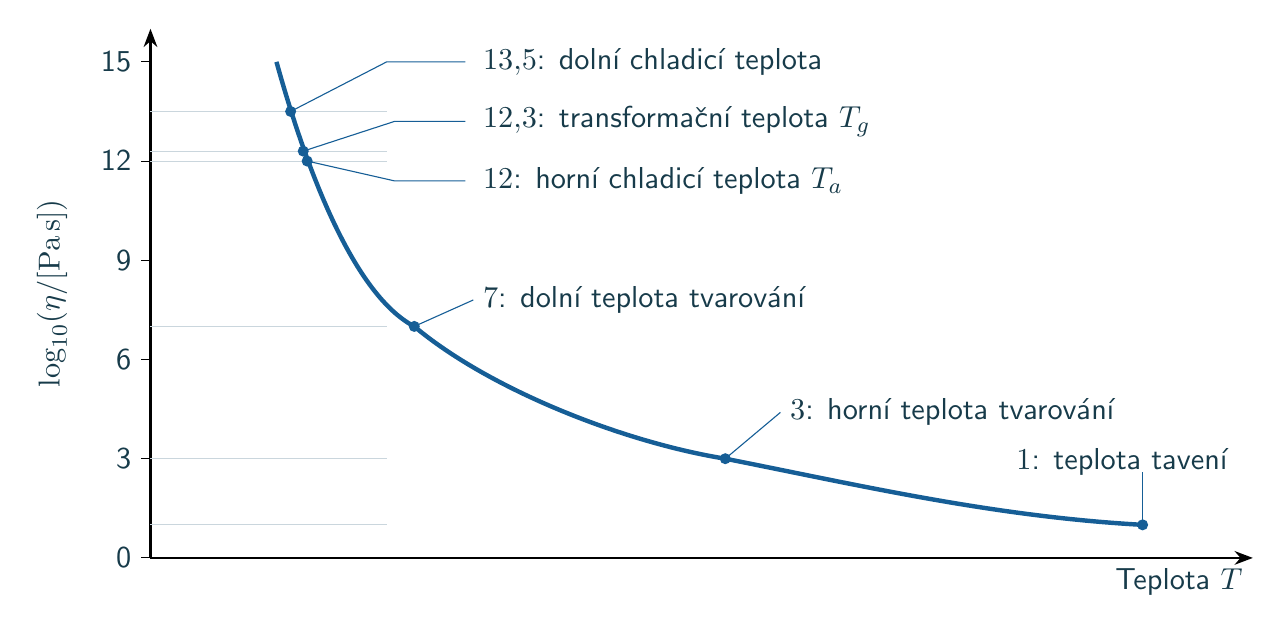
\begin{tikzpicture}[x=1cm,y=.42cm,font=\sffamily\fontsize{11}{13}\selectfont,>=Stealth,text=ink]
\draw[->,line width=.8pt] (0,0)--(14,0) node[below left] {Teplota $T$};
\draw[->,line width=.8pt] (0,0)--(0,16);
\node[rotate=90] at (-1.25,8) {$\log_{10}\!\left(\eta/[\mathrm{Pa\,s}]\right)$};
\foreach \y/\label in {1/1,3/3,7/7,12/12,12.3/{12{,}3},13.5/{13{,}5}}{
 \draw[guide] (0,\y)--(3,\y);
}
\draw[curve,line width=1.6pt] (1.6,15)
 ..controls (1.95,12) and (2.55,8)..(3.35,7)
 ..controls (4.3,5.1) and (6,3.5)..(7.3,3)
 ..controls (9,2.2) and (10.7,1.25)..(12.6,1);
% Vytažené popisky těsně sousedících bodů zůstávají navzájem oddělené.
\fill[curve] (1.78,13.5) circle (2pt);
\draw[curve] (1.78,13.5)--(3,15)--(4,15);
\node[anchor=west] at (4.1,15) {$13{,}5$: dolní chladicí teplota};
\fill[curve] (1.94,12.3) circle (2pt);
\draw[curve] (1.94,12.3)--(3.1,13.2)--(4,13.2);
\node[anchor=west] at (4.1,13.2) {$12{,}3$: transformační teplota $T_g$};
\fill[curve] (1.99,12) circle (2pt);
\draw[curve] (1.99,12)--(3.1,11.4)--(4,11.4);
\node[anchor=west] at (4.1,11.4) {$12$: horní chladicí teplota $T_a$};
\fill[curve] (3.35,7) circle (2pt);
\draw[curve] (3.35,7)--(4.1,7.8);
\node[anchor=west] at (4.1,7.8) {$7$: dolní teplota tvarování};
\fill[curve] (7.3,3) circle (2pt);
\draw[curve] (7.3,3)--(8,4.4);
\node[anchor=west] at (8,4.4) {$3$: horní teplota tvarování};
\fill[curve] (12.6,1) circle (2pt);
\draw[curve] (12.6,1)--(12.6,2.6);
\node[anchor=east] at (13.8,2.9) {$1$: teplota tavení};
\foreach \y in {0,3,6,9,12,15}{\draw (0,\y)--(-.12,\y) node[left]{\y};}
\end{tikzpicture}
\end{document}
